%%
%% Automatically generated file from DocOnce source
%% (https://github.com/doconce/doconce/)
%% doconce format html main_pandas.do.txt CHAPTER=document BOOK=document APPENDIX=document --latex_todonotes --device=screen --latex_admon_color=1,1,1 --latex_admon=mdfbox --latex_list_of_exercises=toc --latex_table_format=left --latex_code_style=default:vrb-blue1@sys:vrb[frame=lines,label=\fbox{{\tiny Terminal}},framesep=2.5mm,framerule=0.7pt]

% #define PREAMBLE

% #ifdef PREAMBLE
%-------------------- begin preamble ----------------------

\documentclass[%
oneside,                 % oneside: electronic viewing, twoside: printing
final,                   % draft: marks overfull hboxes, figures with paths
10pt]{article}

\listfiles               %  print all files needed to compile this document

\usepackage{relsize,makeidx,color,setspace,amsmath,amsfonts,amssymb}
\usepackage[table]{xcolor}
\usepackage{bm,ltablex,microtype}

\usepackage[pdftex]{graphicx}

% Packages for typesetting blocks of computer code
\usepackage{fancyvrb,framed,moreverb}

% Define colors
\definecolor{orange}{cmyk}{0,0.4,0.8,0.2}
\definecolor{tucorange}{rgb}{1.0,0.64,0}
\definecolor{darkorange}{rgb}{.71,0.21,0.01}
\definecolor{darkgreen}{rgb}{.12,.54,.11}
\definecolor{myteal}{rgb}{.26, .44, .56}
\definecolor{gray}{gray}{0.45}
\definecolor{mediumgray}{gray}{.8}
\definecolor{lightgray}{gray}{.95}
\definecolor{brown}{rgb}{0.54,0.27,0.07}
\definecolor{purple}{rgb}{0.5,0.0,0.5}
\definecolor{darkgray}{gray}{0.25}
\definecolor{darkblue}{rgb}{0,0.08,0.45}
\definecolor{darkblue2}{rgb}{0,0,0.8}
\definecolor{lightred}{rgb}{1.0,0.39,0.28}
\definecolor{lightgreen}{rgb}{0.48,0.99,0.0}
\definecolor{lightblue}{rgb}{0.53,0.81,0.92}
\definecolor{lightblue2}{rgb}{0.3,0.3,1.0}
\definecolor{lightpurple}{rgb}{0.87,0.63,0.87}
\definecolor{lightcyan}{rgb}{0.5,1.0,0.83}

\colorlet{comment_green}{green!50!black}
\colorlet{string_red}{red!60!black}
\colorlet{keyword_pink}{magenta!70!black}
\colorlet{indendifier_green}{green!70!white}

% Backgrounds for code
\definecolor{cbg_gray}{rgb}{.95, .95, .95}
\definecolor{bar_gray}{rgb}{.92, .92, .92}

\definecolor{cbg_yellowgray}{rgb}{.95, .95, .85}
\definecolor{bar_yellowgray}{rgb}{.95, .95, .65}

\colorlet{cbg_yellow2}{yellow!10}
\colorlet{bar_yellow2}{yellow!20}

\definecolor{cbg_yellow1}{rgb}{.98, .98, 0.8}
\definecolor{bar_yellow1}{rgb}{.98, .98, 0.4}

\definecolor{cbg_red1}{rgb}{1, 0.85, 0.85}
\definecolor{bar_red1}{rgb}{1, 0.75, 0.85}

\definecolor{cbg_blue1}{rgb}{0.87843, 0.95686, 1.0}
\definecolor{bar_blue1}{rgb}{0.7,     0.95686, 1}

%\setlength{\fboxsep}{-1.5mm}  % adjust cod_vpad/pro_vpad background box

%% Background for code blocks (parameter is color name)

%% pro/cod_vpad: gives some vertical padding before and after the text
%% (but has more simplistic code than _cod/pro_tight+cod/pro).
%% pro/cod_vpad can be used to enclose Verbatim or lst begin/end for code.
%% pro/cod calls _pro/cod_tight and has very little vertical padding,
%% used to enclose Verbatim and other begin/end for code.
%% (pro/cod is what the ptex2tex program could produce with the
%% Blue/BlueBar definitions in .ptex2tex.cfg.)

\newenvironment{cod_vpad}[1]{
   \def\FrameCommand{\colorbox{#1}}
   \MakeFramed{\FrameRestore}}
   {\endMakeFramed}

\newenvironment{_cod_tight}[1]{
   \def\FrameCommand{\colorbox{#1}}
   \FrameRule0.6pt\MakeFramed {\FrameRestore}\vskip3mm}
   {\vskip0mm\endMakeFramed}

\newenvironment{cod}[1]{
\bgroup\rmfamily
\fboxsep=0mm\relax
\begin{_cod_tight}{#1}
\list{}{\parsep=-2mm\parskip=0mm\topsep=0pt\leftmargin=2mm
\rightmargin=2\leftmargin\leftmargin=4pt\relax}
\item\relax}
{\endlist\end{_cod_tight}\egroup}

%% Background for complete program blocks (parameter 1 is color name
%% for background, parameter 2 is color for left bar)
\newenvironment{pro_vpad}[2]{
   \def\FrameCommand{\color{#2}\vrule width 1mm\normalcolor\colorbox{#1}}
   \MakeFramed{\FrameRestore}}
   {\endMakeFramed}

\newenvironment{_pro_tight}[2]{
   \def\FrameCommand{\color{#2}\vrule width 1mm\normalcolor\colorbox{#1}}
   \FrameRule0.6pt\MakeFramed {\advance\hsize-2mm\FrameRestore}\vskip3mm}
   {\vskip0mm\endMakeFramed}

\newenvironment{pro}[2]{
\bgroup\rmfamily
\fboxsep=0mm\relax
\begin{_pro_tight}{#1}{#2}
\list{}{\parsep=-2mm\parskip=0mm\topsep=0pt\leftmargin=2mm
\rightmargin=2\leftmargin\leftmargin=4pt\relax}
\item\relax}
{\endlist\end{_pro_tight}\egroup}


\usepackage[T1]{fontenc}
%\usepackage[latin1]{inputenc}
\usepackage{ucs}
\usepackage[utf8x]{inputenc}

\usepackage{lmodern}         % Latin Modern fonts derived from Computer Modern

% Hyperlinks in PDF:
\definecolor{linkcolor}{rgb}{0,0,0.4}
\usepackage{hyperref}
\hypersetup{
    breaklinks=true,
    colorlinks=true,
    linkcolor=linkcolor,
    urlcolor=linkcolor,
    citecolor=black,
    filecolor=black,
    %filecolor=blue,
    pdfmenubar=true,
    pdftoolbar=true,
    bookmarksdepth=3   % Uncomment (and tweak) for PDF bookmarks with more levels than the TOC
    }
%\hyperbaseurl{}   % hyperlinks are relative to this root

\setcounter{tocdepth}{2}  % levels in table of contents

% Tricks for having figures close to where they are defined:
% 1. define less restrictive rules for where to put figures
\setcounter{topnumber}{2}
\setcounter{bottomnumber}{2}
\setcounter{totalnumber}{4}
\renewcommand{\topfraction}{0.95}
\renewcommand{\bottomfraction}{0.95}
\renewcommand{\textfraction}{0}
\renewcommand{\floatpagefraction}{0.75}
% floatpagefraction must always be less than topfraction!
% 2. ensure all figures are flushed before next section
\usepackage[section]{placeins}
% 3. enable begin{figure}[H] (often leads to ugly pagebreaks)
%\usepackage{float}\restylefloat{figure}

\usepackage[framemethod=TikZ]{mdframed}

% --- begin definitions of admonition environments ---

% Admonition style "mdfbox" is an oval colored box based on mdframed
% "notice" admon
\definecolor{mdfbox_notice_background}{rgb}{1,1,1}
\newmdenv[
  skipabove=15pt,
  skipbelow=15pt,
  outerlinewidth=0,
  backgroundcolor=mdfbox_notice_background,
  linecolor=black,
  linewidth=2pt,       % frame thickness
  frametitlebackgroundcolor=blue!5,
  frametitlerule=true,
  frametitlefont=\normalfont\bfseries,
  shadow=false,        % frame shadow?
  shadowsize=11pt,
  leftmargin=0,
  rightmargin=0,
  roundcorner=5,
  needspace=0pt,
]{notice_mdfboxmdframed}

\newenvironment{notice_mdfboxadmon}[1][]{
\begin{notice_mdfboxmdframed}[frametitle=#1]
}
{
\end{notice_mdfboxmdframed}
}

% Admonition style "mdfbox" is an oval colored box based on mdframed
% "summary" admon
\definecolor{mdfbox_summary_background}{rgb}{1,1,1}
\newmdenv[
  skipabove=15pt,
  skipbelow=15pt,
  outerlinewidth=0,
  backgroundcolor=mdfbox_summary_background,
  linecolor=black,
  linewidth=2pt,       % frame thickness
  frametitlebackgroundcolor=blue!5,
  frametitlerule=true,
  frametitlefont=\normalfont\bfseries,
  shadow=false,        % frame shadow?
  shadowsize=11pt,
  leftmargin=0,
  rightmargin=0,
  roundcorner=5,
  needspace=0pt,
]{summary_mdfboxmdframed}

\newenvironment{summary_mdfboxadmon}[1][]{
\begin{summary_mdfboxmdframed}[frametitle=#1]
}
{
\end{summary_mdfboxmdframed}
}

% Admonition style "mdfbox" is an oval colored box based on mdframed
% "warning" admon
\definecolor{mdfbox_warning_background}{rgb}{1,1,1}
\newmdenv[
  skipabove=15pt,
  skipbelow=15pt,
  outerlinewidth=0,
  backgroundcolor=mdfbox_warning_background,
  linecolor=black,
  linewidth=2pt,       % frame thickness
  frametitlebackgroundcolor=blue!5,
  frametitlerule=true,
  frametitlefont=\normalfont\bfseries,
  shadow=false,        % frame shadow?
  shadowsize=11pt,
  leftmargin=0,
  rightmargin=0,
  roundcorner=5,
  needspace=0pt,
]{warning_mdfboxmdframed}

\newenvironment{warning_mdfboxadmon}[1][]{
\begin{warning_mdfboxmdframed}[frametitle=#1]
}
{
\end{warning_mdfboxmdframed}
}

% Admonition style "mdfbox" is an oval colored box based on mdframed
% "question" admon
\definecolor{mdfbox_question_background}{rgb}{1,1,1}
\newmdenv[
  skipabove=15pt,
  skipbelow=15pt,
  outerlinewidth=0,
  backgroundcolor=mdfbox_question_background,
  linecolor=black,
  linewidth=2pt,       % frame thickness
  frametitlebackgroundcolor=blue!5,
  frametitlerule=true,
  frametitlefont=\normalfont\bfseries,
  shadow=false,        % frame shadow?
  shadowsize=11pt,
  leftmargin=0,
  rightmargin=0,
  roundcorner=5,
  needspace=0pt,
]{question_mdfboxmdframed}

\newenvironment{question_mdfboxadmon}[1][]{
\begin{question_mdfboxmdframed}[frametitle=#1]
}
{
\end{question_mdfboxmdframed}
}

% Admonition style "mdfbox" is an oval colored box based on mdframed
% "block" admon
\definecolor{mdfbox_block_background}{rgb}{1,1,1}
\newmdenv[
  skipabove=15pt,
  skipbelow=15pt,
  outerlinewidth=0,
  backgroundcolor=mdfbox_block_background,
  linecolor=black,
  linewidth=2pt,       % frame thickness
  frametitlebackgroundcolor=blue!5,
  frametitlerule=true,
  frametitlefont=\normalfont\bfseries,
  shadow=false,        % frame shadow?
  shadowsize=11pt,
  leftmargin=0,
  rightmargin=0,
  roundcorner=5,
  needspace=0pt,
]{block_mdfboxmdframed}

\newenvironment{block_mdfboxadmon}[1][]{
\begin{block_mdfboxmdframed}[frametitle=#1]
}
{
\end{block_mdfboxmdframed}
}

% --- end of definitions of admonition environments ---

% prevent orhpans and widows
\clubpenalty = 10000
\widowpenalty = 10000

% --- end of standard preamble for documents ---


% insert custom LaTeX commands...

\raggedbottom
\makeindex
\usepackage[totoc]{idxlayout}   % for index in the toc
\usepackage[nottoc]{tocbibind}  % for references/bibliography in the toc

%-------------------- end preamble ----------------------

\begin{document}

% matching end for #ifdef PREAMBLE
% #endif

\newcommand{\exercisesection}[1]{\subsection*{#1}}

% This file is to be run by preprocess to produce newcommands.tex
% to be included in .tex files.
% There are format-specific tests here for the newcommands (i.e.,
% different definitions of the commands depending on latex or mathjax).

% Newcommands for LaTeX math.
\newcommand{\no}{\nonumber}
\newcommand{\tp}{\thinspace .}
\renewcommand{\Re}{\bbbr}
\newcommand{\Oof}[1]{\mathcal{O}(#1)}
\newcommand{\Prob}[1]{\hbox{P}(#1)}
\newcommand{\Var}[1]{\hbox{Var}(#1)}
\newcommand{\Cov}[2]{\hbox{Cov}(#1,#2)}
\newcommand{\StDev}[1]{\hbox{StDev}(#1)}
\newcommand{\co}{CO$_2$}

% Use footnotesize in subscripts
\newcommand{\subsc}[2]{#1_{\mbox{\footnotesize #2}}}




% ------------------- main content ----------------------



% ----------------- title -------------------------

\thispagestyle{empty}

\begin{center}
{\LARGE\bf
\begin{spacing}{1.25}
Organizing data: pandas
\end{spacing}
}
\end{center}

% ----------------- author(s) -------------------------

\begin{center}
{\bf Aksel Hiorth${}^{}$} \\ [0mm]
\end{center}

\begin{center}
% List of all institutions:
\end{center}
    
% ----------------- end author(s) -------------------------
University of Stavanger

% --- begin date ---
\begin{center}
Mar 26, 2023
\end{center}
% --- end date ---

\vspace{1cm}


\tableofcontents

\vspace{1cm} % after toc

% Common Mako variables and functions

\section{What is Pandas?}
Pandas is a Python package that among many things are used to handle data, and perform operations on groups of data. It is built on top of Numpy, which makes it easy to perform vectorized operations. Pandas is written by Wes McKinney, and one of it objectives is according to the official website \href{{https://pandas.pydata.org/}}{'' providing fast, flexible, and expressive data structures designed to make working with ''relational'' or ''labeled'' data both easy and intuitive. It aims to be the fundamental high-level building block for doing practical, real-world data analysis in Python''}. Pandas also has excellent functions for reading and writing excel and csv files.  An excel file is read directly into memory in what is called a \texttt{DataFrame} in Pandas. A DataFrame is a two dimensional object where data are typically stored in column or row format. Pandas has a lot of functions that can be used to calculate statistical properties of the data frame as a whole. In this chapter we will focus on basic data manipulation, stuff you might do in excel, but can be done much faster in Python and Pandas.

\section{Creating a data frame}
In the following we will assume that you have imported pandas, like this


\begin{pro}{cbg_blue1}{bar_blue1}\begin{Verbatim}[numbers=none,fontsize=\fontsize{9pt}{9pt},baselinestretch=0.95,xleftmargin=2mm]
import pandas as pd

\end{Verbatim}
\end{pro}
\noindent


\subsection{From empty DataFrame}
This is perhaps the most basic way of creating a DataFrame, first we create an empty DataFrame


\begin{pro}{cbg_blue1}{bar_blue1}\begin{Verbatim}[numbers=none,fontsize=\fontsize{9pt}{9pt},baselinestretch=0.95,xleftmargin=2mm]
df = pd.DataFrame()

\end{Verbatim}
\end{pro}
\noindent


\begin{notice_mdfboxadmon}[Variable name.]
Note that we often use \texttt{df} as a variable name for a DataFrame, this is a choice, but it is a usually a good choice as someone else reading the code could infer from a name that \texttt{df} is a DataFrame. If you need more than one DataFrame variable you could use \texttt{df1}, \texttt{df2}, etc. or even better to use a descriptive name, \Verb!df_sales_data!.
\end{notice_mdfboxadmon} % title: Variable name.


Next, we can add columns to the DataFrame






\begin{pro}{cbg_blue1}{bar_blue1}\begin{Verbatim}[numbers=none,fontsize=\fontsize{9pt}{9pt},baselinestretch=0.95,xleftmargin=2mm]
df=pd.DataFrame()
df['ints']=[0,1,2,3]
df['floats']=[4.,5.,6.,7.]
df['tools']=['hammer','saw','rock','nail']
print(df) # to view data frame

\end{Verbatim}
\end{pro}
\noindent

Note that all columns needs to have the same size.


\begin{notice_mdfboxadmon}[\texttt{pd.Series()}.]
Even if we initialize the DataFrame column with a list, the command \texttt{type(df['a'])} will tell you that the column in the DataFrame are of type \texttt{pd.Series()}. Thus the fundamental objects in Pandas are of type \texttt{Series}. Series are more flexible, and it is possible to calculate \texttt{df['a']/df['b']}, whereas \texttt{[0,1,2,3]/[4,5,6,7]} is not possible.
\end{notice_mdfboxadmon} % title: \texttt{pd.Series()}.



\subsection{Create DataFrame from dictionary}
A DataFrame can be quite easily be generated from a dictionary. A dictionary is a special data structure, where an unique key is associated with a data type (key:value pair). In this case, the key would be the title of the column, and the value would be the data in the columns.







\begin{pro}{cbg_blue1}{bar_blue1}\begin{Verbatim}[numbers=none,fontsize=\fontsize{9pt}{9pt},baselinestretch=0.95,xleftmargin=2mm]
my_dict={'ints':[0,1,2,3], 'floats':[4.,5.,6.,7.],
'tools':['hammer','saw','rock','nail']
}
df=pd.DataFrame(my_dict)
print(df) # to view

\end{Verbatim}
\end{pro}
\noindent


\subsection{From file}
Assume you have some data organized in excel or in a csv file. The csv file could just be a file with column data, they could be separated by a comma or tab

\begin{figure}[!ht]  % fig:file
  \centerline{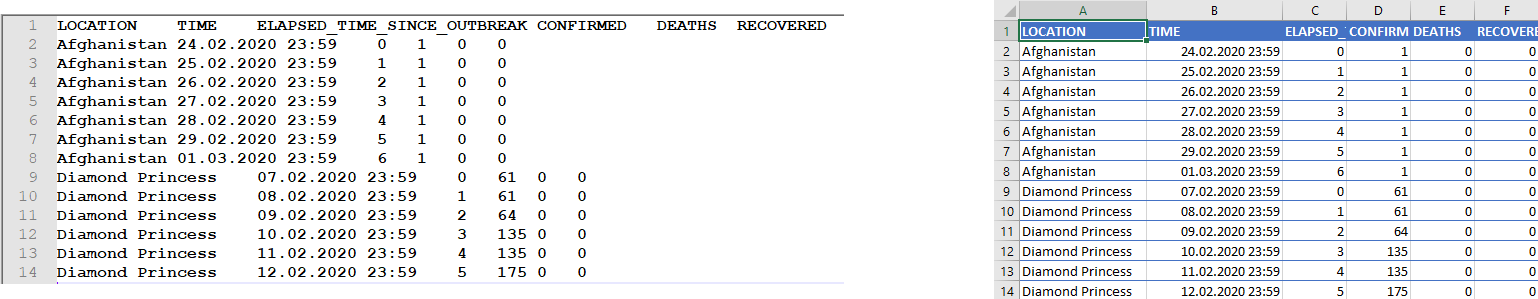
\includegraphics[width=1.0\linewidth]{fig-pandas/covid_comb.png}}
  \caption{
  Official Covid-19 data, and example of files (left) tab separated (right) excel file. \label{fig:file}
  }
\end{figure}
%\clearpage % flush figures fig:file




\begin{pro}{cbg_blue1}{bar_blue1}\begin{Verbatim}[numbers=none,fontsize=\fontsize{9pt}{9pt},baselinestretch=0.95,xleftmargin=2mm]
df=pd.read_excel('../data/corona_data.xlsx') # excel file
df2=pd.read_csv('../data/corona_data.dat',sep='\t') # csv tab separated file

\end{Verbatim}
\end{pro}
\noindent

If the excel file has several sheets, you can give the sheet name directly, e.g. \Verb!df=pd.read_excel('file.xlsx',sheet_name="Sheet1")!, for more information see the \href{{https://pandas.pydata.org/docs/reference/api/pandas.read_excel.html}}{documentation}. 


\begin{notice_mdfboxadmon}[Accessing files.]
Accessing files from python can be painful. If excel files are open in excel, Windows will not allow a different program to access it - always remember to close the file before opening it. Sometimes we are not in the right directory, to check which directory you are in, you can always do the following



\begin{pro}{cbg_blue1}{bar_blue1}\begin{Verbatim}[numbers=none,fontsize=\fontsize{9pt}{9pt},baselinestretch=0.95,xleftmargin=2mm]
import os
print(os.getcwd()) # prints current working directory

\end{Verbatim}
\end{pro}
\noindent
\end{notice_mdfboxadmon} % title: Accessing files.



We can easily save the data frame to excel format and open it in excel


\begin{pro}{cbg_blue1}{bar_blue1}\begin{Verbatim}[numbers=none,fontsize=\fontsize{9pt}{9pt},baselinestretch=0.95,xleftmargin=2mm]
df.to_excel('covid19.xlsx', index=False) # what happens if you put index=True?

\end{Verbatim}
\end{pro}
\noindent



\begin{notice_mdfboxadmon}[Index column.]
Whenever you create a DataFrame Pandas by default create an index column, it contains an integer for each row starting at zero. It can be accessed by \texttt{df.index}, and it is also possible to define another column as index column.
\end{notice_mdfboxadmon} % title: Index column.



\subsection{Accessing data in  DataFrames}

\paragraph{Selecting columns.}
If we want to pick out a specific column we can access it in the following ways







\begin{pro}{cbg_blue1}{bar_blue1}\begin{Verbatim}[numbers=none,fontsize=\fontsize{9pt}{9pt},baselinestretch=0.95,xleftmargin=2mm]
# following two are equivalent
time=df['TIME'] # by the name, alternatively
time=df[df.columns[1]]
# following two are equivalent
time=df.loc[:,['TIME']] # by loc[] if we use name
time=df.iloc[:,1] # by iloc, pick column number 1

\end{Verbatim}
\end{pro}
\noindent

The \texttt{loc[]} and \texttt{iloc[]} functions also allows for list slicing, one can then pick e.g.~every second element in the column by \texttt{time=df.iloc[::2,1]} etc. The difference is that \texttt{loc[]} uses the name, and \texttt{iloc[]} the index (usually an integer). 

Why several ways of doing the same operation? It turns out that although we are able to extract what we want with these operations, they are of different type



\begin{pro}{cbg_blue1}{bar_blue1}\begin{Verbatim}[numbers=none,fontsize=\fontsize{9pt}{9pt},baselinestretch=0.95,xleftmargin=2mm]
print(type(df['TIME']))
print(type(df.loc[:,['TIME']]))

\end{Verbatim}
\end{pro}
\noindent

\paragraph{Selecting rows.}
When selecting rows in a DataFrame, we can use the \texttt{loc[]} and \texttt{iloc[]} functions




\begin{pro}{cbg_blue1}{bar_blue1}\begin{Verbatim}[numbers=none,fontsize=\fontsize{9pt}{9pt},baselinestretch=0.95,xleftmargin=2mm]
# pick column number 0 and 1
time=df.loc[0:1,:] # by loc[] 
time=df.iloc[0:2,:] # by iloc

\end{Verbatim}
\end{pro}
\noindent



\begin{notice_mdfboxadmon}[\texttt{pandas.DataFrame.loc} vs \texttt{pandas.DataFrame.iloc}.]
When selecting rows \texttt{loc} and \texttt{iloc} they behave differently, \texttt{loc} includes the endpoints (in the example above both row 0 and 1), whereas \texttt{iloc} includes the starting point and up to 1 minus the endpoint.
\end{notice_mdfboxadmon} % title: \texttt{pandas.DataFrame.loc} vs \texttt{pandas.DataFrame.iloc}.



\paragraph{Challenges when accessing columns or rows.}

\begin{notice_mdfboxadmon}[Special characters.]
Sometimes when reading files from excel, headers may contains invisible characters like newline \Verb!\n! or tab \Verb!\t! or maybe Norwegian special letters that have not been read in properly. If you have problem accessing a column by name do \texttt{print(df.columns)} and check if the name matches what you would expect.
\end{notice_mdfboxadmon} % title: Special characters.



If the header names has unwanted white space, one can do





\begin{pro}{cbg_blue1}{bar_blue1}\begin{Verbatim}[numbers=none,fontsize=\fontsize{9pt}{9pt},baselinestretch=0.95,xleftmargin=2mm]
df.columns = df.columns.str.replace(' ', '') # all white spaces
df.columns = df.columns.str.lstrip() # the beginning of string
df.columns = df.columns.str.rstrip() # end of string
df.columns = df.columns.str.strip()  # both ends

\end{Verbatim}
\end{pro}
\noindent

Similarly for unwanted tabs


\begin{pro}{cbg_blue1}{bar_blue1}\begin{Verbatim}[numbers=none,fontsize=\fontsize{9pt}{9pt},baselinestretch=0.95,xleftmargin=2mm]
df.columns = df.columns.str.replace('\t', '') # remove tab

\end{Verbatim}
\end{pro}
\noindent

If you want to make sure that the columns does not contain any white spaces, one can use \href{{https://pandas.pydata.org/pandas-docs/version/1.2.4/reference/api/pandas.Series.str.strip.html}}{\nolinkurl{pandas.Series.str.strip()}}


\begin{pro}{cbg_blue1}{bar_blue1}\begin{Verbatim}[numbers=none,fontsize=\fontsize{9pt}{9pt},baselinestretch=0.95,xleftmargin=2mm]
df['LOCATION']=df['LOCATION'].str.strip()

\end{Verbatim}
\end{pro}
\noindent


\paragraph{Time columns not parsed properly.}
If you have dates in the file (as in our case for the \texttt{TIME} column), you should check if they are in the \texttt{datetime} format and not read as \texttt{str}.


\begin{notice_mdfboxadmon}[\texttt{datetime}.]
The \texttt{datetime} library is very useful for working with dates. Data types of the type \texttt{datetime} (or equivalently \texttt{timestamp} used by Pandas) contains both date and time in the format \texttt{YYYY-MM-DD hh:mm:ss}. We can initialize a variable, \texttt{a}, by \texttt{a=datetime.datetime(2022,8,30,10,14,1)}, to access the hour we do \texttt{a.hour}, the year by \texttt{a.year} etc. It also easy to increase e.g.~the day by one by doing \texttt{a+datetime.timedelta(days=1)}.
\end{notice_mdfboxadmon} % title: \texttt{datetime}.










\begin{pro}{cbg_blue1}{bar_blue1}\begin{Verbatim}[numbers=none,fontsize=\fontsize{9pt}{9pt},baselinestretch=0.95,xleftmargin=2mm]
import datetime as dt
time=df['TIME']
# what happens if you set
# time=df2['TIME'] #i.e df2 is from pd.read_csv ?
print(time[0])
print(time[0]+dt.timedelta(days=1))

\end{Verbatim}
\end{pro}
\noindent


The code above might work fine or in some cases a date is parsed as a string by Pandas, then we need to convert that column to the correct format. If not, we get into problems if you want to plot data vs the time column.

Below are two ways of converting the \texttt{TIME} column






\begin{pro}{cbg_blue1}{bar_blue1}\begin{Verbatim}[numbers=none,fontsize=\fontsize{9pt}{9pt},baselinestretch=0.95,xleftmargin=2mm]
df2['TIME']=pd.to_datetime(df2['TIME'])
# just for testing that everything went ok
time=df2['TIME']
print(time[0])
print(time[0]+dt.timedelta(days=1))

\end{Verbatim}
\end{pro}
\noindent


Another possibility is to do the conversion when reading the data:


\begin{pro}{cbg_blue1}{bar_blue1}\begin{Verbatim}[numbers=none,fontsize=\fontsize{9pt}{9pt},baselinestretch=0.95,xleftmargin=2mm]
df2=pd.read_csv('../data/corona_data.dat',sep='\t',parse_dates=['TIME']) 

\end{Verbatim}
\end{pro}
\noindent

If you have a need to specify all data types, to avoid potential problems down the line this can also be done. First create a dictionary, with column names and data types



\begin{pro}{cbg_blue1}{bar_blue1}\begin{Verbatim}[numbers=none,fontsize=\fontsize{9pt}{9pt},baselinestretch=0.95,xleftmargin=2mm]
types_dict={"LOCATION":str,"TIME":str,"ELAPSED_TIME_SINCE_OUTBREAK":int,"CONFIRMED":int,"DEATHS":int,"RECOVERED":int}
df2=pd.read_csv('../data/corona_data.dat',sep='\t',dtype=types_dict,parse_dates=['TIME']) # set data types explicit

\end{Verbatim}
\end{pro}
\noindent

Note that the time data type is \texttt{str}, but we explicitly tell Pandas to convert those to \texttt{datetime}.

\subsection{Filtering and visualizing data}
\paragraph{Boolean masking.}
Typically you would select rows based on a criterion, the syntax in Pandas is that you enter a series containing \texttt{True} and \texttt{False} for the rows you want to pick out, e.g.~to pick out all entries with Afghanistan we can do


\begin{pro}{cbg_blue1}{bar_blue1}\begin{Verbatim}[numbers=none,fontsize=\fontsize{9pt}{9pt},baselinestretch=0.95,xleftmargin=2mm]
df[df['LOCATION'] == 'Afghanistan']

\end{Verbatim}
\end{pro}
\noindent

The innermost statement \texttt{df['LOCATION'] == 'Afghanistan'} gives a logical vector with the value \texttt{True} for the five last elements and \texttt{False} for the rest. Then we pass this to the DataFrame, and in one go the unwanted elements are removed. It is also possible to use several criteria, e.g.~only extracting data after a specific time


\begin{pro}{cbg_blue1}{bar_blue1}\begin{Verbatim}[numbers=none,fontsize=\fontsize{9pt}{9pt},baselinestretch=0.95,xleftmargin=2mm]
df[(df['LOCATION'] == 'Afghanistan') & (df['ELAPSED_TIME_SINCE_OUTBREAK'] > 2)]

\end{Verbatim}
\end{pro}
\noindent

Note that the parenthesis are necessary, otherwise the logical operation would fail.

\paragraph{Plotting a DataFrame.}
Pandas has built in plotting, by calling \href{{https://pandas.pydata.org/docs/reference/api/pandas.DataFrame.plot.html}}{\nolinkurl{pandas.DataFrame.plot}}.







\begin{pro}{cbg_blue1}{bar_blue1}\begin{Verbatim}[numbers=none,fontsize=\fontsize{9pt}{9pt},baselinestretch=0.95,xleftmargin=2mm]
df2=df[(df['LOCATION'] == 'Afghanistan')]
df2.plot()
#try 
#df2=df2.set_index('TIME')
#df2.plot() # what is the difference?
#df2.plot(y=['CONFIRMED','DEATHS'])

\end{Verbatim}
\end{pro}
\noindent

\subsection{Performing mathematical operations on DataFrames}
When performing mathematical operations on DataFrames there are at least two strategies
\begin{itemize}
\item Extract columns from the DataFrame and perform mathematical operations on the columns using Numpy, leaving the original DataFrame intact

\item To operate directly on the data in the DataFrame using the Pandas library
\end{itemize}

\noindent

\begin{notice_mdfboxadmon}[Speed and performance.]
Using Pandas or Numpy should in principle be equally fast. The advice is to not worry about performance before it is necessary. Use the methods you are confident with, and try to be consistent. By consistent, we mean that if you have found one way of doing a certain operation stick to that one and try not to implement many different ways of doing the same thing.
\end{notice_mdfboxadmon} % title: Speed and performance.



We can always access the individual columns in a DataFrame by the syntax \Verb!df['column_name']!. 
\paragraph{Example: mathematical operations on DataFrames.}
\begin{enumerate}
\item Create a DataFrame with one column (\texttt{a}) containing ten thousand random uniformly distributed numbers between 0 and 1 (checkout \href{{https://numpy.org/doc/stable/reference/random/generated/numpy.random.uniform.html}}{\nolinkurl{np.random.uniform}})

\item Add two new columns: one which all elements of \texttt{a} is squared and one where the sine function is applied to column \texttt{a}

\item Calculate the inverse of all the numbers in the DataFrame

\item Make a plot of the results (i.e. \texttt{a} vs \texttt{a*a}, and \texttt{a} vs \texttt{sin(a)})
\end{enumerate}

\noindent
\paragraph{Solution.}
\begin{enumerate}
\item First we make the DataFrame
\end{enumerate}

\noindent







\begin{pro}{cbg_blue1}{bar_blue1}\begin{Verbatim}[numbers=none,fontsize=\fontsize{9pt}{9pt},baselinestretch=0.95,xleftmargin=2mm]
import numpy as np
import pandas as pd
N=10000
a=np.random.uniform(0,1,size=N)
df=pd.DataFrame() # empty DataFrame
df['a']=a

\end{Verbatim}
\end{pro}
\noindent

If you like you could also try to use a dictionary. Next, we add the new columns



\begin{pro}{cbg_blue1}{bar_blue1}\begin{Verbatim}[numbers=none,fontsize=\fontsize{9pt}{9pt},baselinestretch=0.95,xleftmargin=2mm]
df['b']=df['a']*df['a'] # alternatively np.square(df['a'])
df['c']=np.sin(df['a'])

\end{Verbatim}
\end{pro}
\noindent


\begin{enumerate}
\item The inverse of all the numbers in the DataFrame can be calculated by simply doing
\end{enumerate}

\noindent


\begin{pro}{cbg_blue1}{bar_blue1}\begin{Verbatim}[numbers=none,fontsize=\fontsize{9pt}{9pt},baselinestretch=0.95,xleftmargin=2mm]
1/df

\end{Verbatim}
\end{pro}
\noindent

Note: you can also do \texttt{df+df} and many other operations on the whole DataFrame.

\begin{enumerate}
\item To make plots there are several possibilities. Personally, I tend most of the time to use the  \href{{https://matplotlib.org/}}{\nolinkurl{matplotlib}} library, simply because I know it quite well, but Pandas has a great deal of very simple methods you can use to generate nice plots with very few commands.
\end{enumerate}

\noindent
\paragraph{Matplotlib:}







\begin{pro}{cbg_blue1}{bar_blue1}\begin{Verbatim}[numbers=none,fontsize=\fontsize{9pt}{9pt},baselinestretch=0.95,xleftmargin=2mm]
import matplotlib.pyplot as plt
plt.plot(df['a'],df['b'], '*', label='$a^2$')
plt.plot(df['a'],df['c'], '^', label='$\sin(a)$')
plt.legend() 
plt.grid() # make small grid lines
plt.show()

\end{Verbatim}
\end{pro}
\noindent


\paragraph{Pandas plotting:}
First, let us try the built in plot command in Pandas


\begin{pro}{cbg_blue1}{bar_blue1}\begin{Verbatim}[numbers=none,fontsize=\fontsize{9pt}{9pt},baselinestretch=0.95,xleftmargin=2mm]
df.plot()

\end{Verbatim}
\end{pro}
\noindent

If you compare this plot with the previous plot, you will see that Pandas plots all columns versus the index columns, which is not what we want. But, we can set \texttt{a} to be the index column



\begin{pro}{cbg_blue1}{bar_blue1}\begin{Verbatim}[numbers=none,fontsize=\fontsize{9pt}{9pt},baselinestretch=0.95,xleftmargin=2mm]
df=df.set_index('a')
df.plot()

\end{Verbatim}
\end{pro}
\noindent

We can also make separate plots


\begin{pro}{cbg_blue1}{bar_blue1}\begin{Verbatim}[numbers=none,fontsize=\fontsize{9pt}{9pt},baselinestretch=0.95,xleftmargin=2mm]
df.plot(subplots=True)

\end{Verbatim}
\end{pro}
\noindent

or scatter plots




\begin{pro}{cbg_blue1}{bar_blue1}\begin{Verbatim}[numbers=none,fontsize=\fontsize{9pt}{9pt},baselinestretch=0.95,xleftmargin=2mm]
df=df.reset_index()
df.plot.scatter(x='a',y='b')
df.plot.scatter(x='a',y='c')

\end{Verbatim}
\end{pro}
\noindent

Note that we have to reset the index, otherwise there are no column named \texttt{a}. 

\subsection{Grouping, filtering and aggregating data}
Whenever you have a data set, you would like to do some exploratory analysis. That typically means that you would like to group, filter or aggregate data. Perhaps, we would like to plot the covid data not per country, but the data as a function of dates. Then you first must sort the data according to date, and then sum all the occurrences on that particular date. For all of these purposes we can use the \href{{https://pandas.pydata.org/docs/reference/api/pandas.DataFrame.groupby.html}}{\nolinkurl{pd.DataFrame.groupby()}} function. To sort our DataFrame on dates and sum the occurrences we can do


\begin{pro}{cbg_blue1}{bar_blue1}\begin{Verbatim}[numbers=none,fontsize=\fontsize{9pt}{9pt},baselinestretch=0.95,xleftmargin=2mm]
df.groupby('TIME').sum()

\end{Verbatim}
\end{pro}
\noindent


Another case could be that we wanted to find the total number of confirmed, deaths and recovered cases in the full database. As always in Python it can be done in different ways, by e.g.~splitting the database into individual countries and do  \texttt{df[['CONFIRMED','DEATHS','RECOVERED']].sum()} or accessing each column individually and sum each of them e.g. \texttt{np.sum(df['CONFIRMED'])}.  However, with the \texttt{groupby()} function
(see figure~\ref{fig:pandas:group} for final result)


\begin{pro}{cbg_blue1}{bar_blue1}\begin{Verbatim}[numbers=none,fontsize=\fontsize{9pt}{9pt},baselinestretch=0.95,xleftmargin=2mm]
df.groupby('LOCATION').sum()

\end{Verbatim}
\end{pro}
\noindent

Here Pandas sum all columns with the same location, and drop columns that cannot be summed. By doing \texttt{df.groupby('LOCATION').mean()} or \texttt{df.groupby('LOCATION').std()} we can find the mean or standard deviation (per day).

\begin{figure}[!ht]  % fig:pandas:group
  \centerline{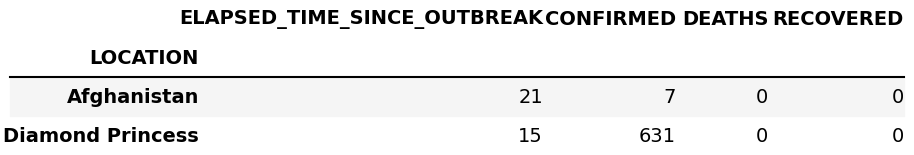
\includegraphics[width=1.0\linewidth]{fig-pandas/group.png}}
  \caption{
  The results of \texttt{df.groupby('LOCATION').sum()}. \label{fig:pandas:group}
  }
\end{figure}
%\clearpage % flush figures fig:pandas:group

\subsection{Simple statistics in Pandas}
At the end it is worth mentioning the built in methods \texttt{pd.DataFrame.mean}, \texttt{pd.DataFrame.median}, \texttt{pd.DataFrame.std} which calculates the mean, median and standard deviation on the columns in the DataFrame where it make sense (i.e.~avoid strings and dates). To get all these values in one go (and a few more) on can also use \texttt{pd.DataFrame.describe()}


\begin{pro}{cbg_blue1}{bar_blue1}\begin{Verbatim}[numbers=none,fontsize=\fontsize{9pt}{9pt},baselinestretch=0.95,xleftmargin=2mm]
df.describe()

\end{Verbatim}
\end{pro}
\noindent

The output is shown in figure~\ref{fig:pandas:desc}

\begin{figure}[!ht]  % fig:pandas:desc
  \centerline{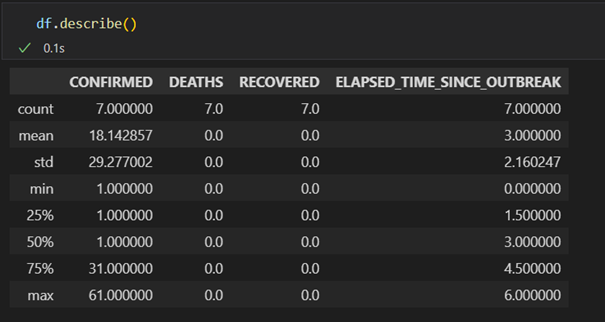
\includegraphics[width=1.0\linewidth]{fig-pandas/describe.png}}
  \caption{
  Output from the describe command. \label{fig:pandas:desc}
  }
\end{figure}
%\clearpage % flush figures fig:pandas:desc

\subsection{Joining two DataFrames}
\paragraph{Appending DataFrames.}
The DataFrame with the Covid-19 data in the previous section could have been created from two separate DataFrames, using \href{{https://pandas.pydata.org/docs/reference/api/pandas.concat.html}}{\nolinkurl{concat()}}. First, create two DataFrames 


















\begin{pro}{cbg_blue1}{bar_blue1}\begin{Verbatim}[numbers=none,fontsize=\fontsize{9pt}{9pt},baselinestretch=0.95,xleftmargin=2mm]
import datetime as dt
a=dt.datetime(2020,2,24,23,59)
b=dt.datetime(2020,2,7,23,59)
my_dict1={'LOCATION':7*['Afghanistan'], 
'TIME':[a+dt.timedelta(days=i) for i in range(7)],
'ELAPSED_TIME_SINCE_OUTBREAK':[0, 1, 2, 3, 4, 5, 6],
'CONFIRMED':7*[1],
'DEATHS':7*[0],
'RECOVERED': 7*[0]}
my_dict2={'LOCATION':6*['Diamond Princess'], 
'TIME':[b+dt.timedelta(days=i) for i in range(6)],
'ELAPSED_TIME_SINCE_OUTBREAK':[0, 1, 2, 3, 4, 5],
'CONFIRMED':[61, 61, 64, 135, 135, 175],
'DEATHS':6*[0],
'RECOVERED': 6*[0]}
df1=pd.DataFrame(my_dict1)
df2=pd.DataFrame(my_dict2)

\end{Verbatim}
\end{pro}
\noindent

Next, add them row wise (see figure~\ref{fig:pandas:concat})




\begin{pro}{cbg_blue1}{bar_blue1}\begin{Verbatim}[numbers=none,fontsize=\fontsize{9pt}{9pt},baselinestretch=0.95,xleftmargin=2mm]
df=pd.concat([df1,df2])
print(df) # to view

\end{Verbatim}
\end{pro}
\noindent


\begin{figure}[!ht]  % fig:pandas:concat
  \centerline{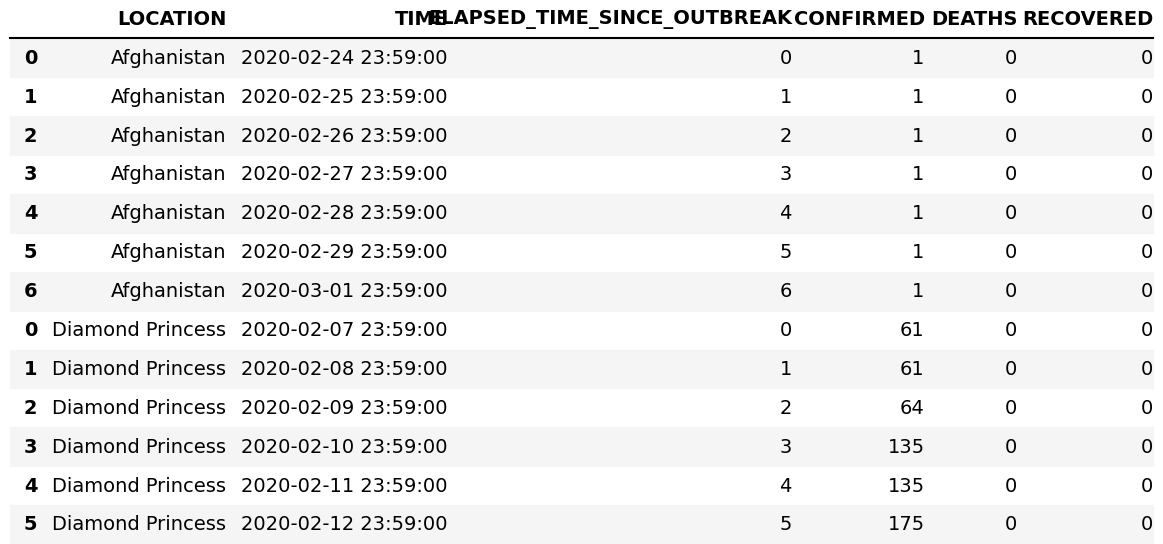
\includegraphics[width=1.0\linewidth]{fig-pandas/concat.png}}
  \caption{
  The result of \texttt{concat()}. \label{fig:pandas:concat}
  }
\end{figure}
%\clearpage % flush figures fig:pandas:concat

If you compare this DataFrame with the previous one, you will see that the index column is different. This is because when joining two DataFrames Pandas does not reset the index by default, doing \Verb!df=pd.concat([df1,df2],ignore_index=True)! resets the index. It is also possible to join DataFrames column vise


\begin{pro}{cbg_blue1}{bar_blue1}\begin{Verbatim}[numbers=none,fontsize=\fontsize{9pt}{9pt},baselinestretch=0.95,xleftmargin=2mm]
pd.concat([df1,df2],axis=1)

\end{Verbatim}
\end{pro}
\noindent


\paragraph{Merging DataFrames.}
In the previous example we had two non overlapping DataFrames (separate countries and times). It could also be the case that some of the data was overlapping e.g.~continuing with the Covid-19 data, one could assume that there was one data set from one region and one from another region in the same country















\begin{pro}{cbg_blue1}{bar_blue1}\begin{Verbatim}[numbers=none,fontsize=\fontsize{9pt}{9pt},baselinestretch=0.95,xleftmargin=2mm]
my_dict1={'LOCATION':7*['Diamond Princess'], 
'TIME':[b+dt.timedelta(days=i) for i in range(7)],
'ELAPSED_TIME_SINCE_OUTBREAK':[0, 1, 2, 3, 4, 5, 6],
'CONFIRMED':7*[1],
'DEATHS':7*[0],
'RECOVERED': 7*[0]}
my_dict2={'LOCATION':2*['Diamond Princess'], 
'TIME':[b+dt.timedelta(days=i) for i in range(2)],
'ELAPSED_TIME_SINCE_OUTBREAK':[0, 1],
'CONFIRMED':[60, 60],
'DEATHS':2*[0],
'RECOVERED': 2*[0]}
df1=pd.DataFrame(my_dict1)
df2=pd.DataFrame(my_dict2)

\end{Verbatim}
\end{pro}
\noindent

If we do \texttt{pd.concat([df1,df2])} we will simply add all values after each other. What we want to do is to sum the number of confirmed, recovered and deaths for the same date. This can be done in several ways, but one way is to use \href{{https://pandas.pydata.org/docs/reference/api/pandas.DataFrame.merge.html}}{\nolinkurl{pd.DataFrame.merge()}}.You can specify the columns to merge on, and choose \texttt{outer} which is union (all data from both frames) or \texttt{inner} which means the intersect (only data which you merge on that exists in both frames), see figure~\ref{fig:pandas:join} for a visual image.

\begin{figure}[!ht]  % fig:pandas:join
  \centerline{
\includegraphics[width=1.0\linewidth]{fig-pandas/fig_join.png}}
  \caption{
  The result of using \texttt{how=outer, inner, left}, or \texttt{right} in \texttt{pd.DataFrame.merge()}. \label{fig:pandas:join}
  }
\end{figure}
%\clearpage % flush figures fig:pandas:join

To be even more specific, after performing the commands



\begin{pro}{cbg_blue1}{bar_blue1}\begin{Verbatim}[numbers=none,fontsize=\fontsize{9pt}{9pt},baselinestretch=0.95,xleftmargin=2mm]
df1.merge(df2,on=['LOCATION','TIME'],how='outer')
df1.merge(df2,on=['LOCATION','TIME'],how='inner')

\end{Verbatim}
\end{pro}
\noindent


we get the results in figure~\ref{fig:pd:merge} 

\begin{figure}[!ht]  % fig:pd:merge
  \centerline{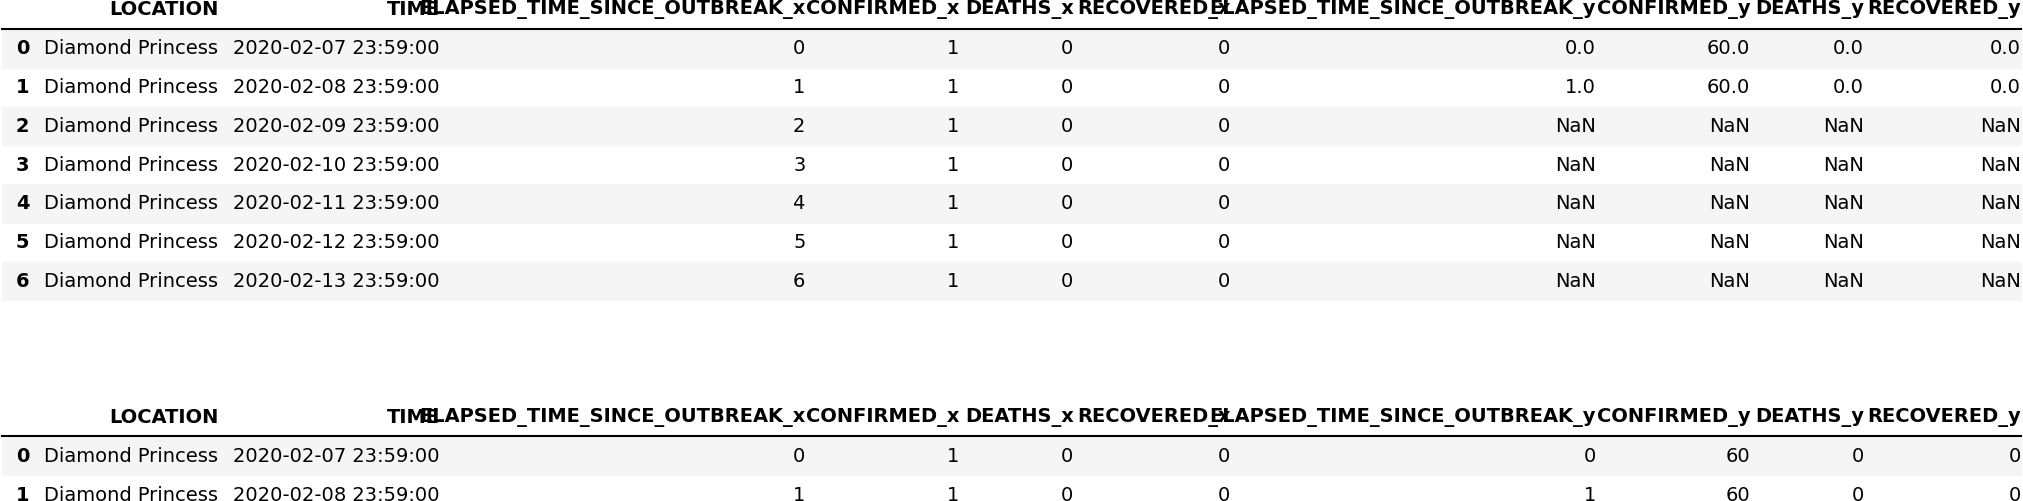
\includegraphics[width=1.0\linewidth]{fig-pandas/merge.png}}
  \caption{
  Merging to dataframes using \texttt{outer} (top) and \texttt{inner} (bottom). \label{fig:pd:merge}
  }
\end{figure}
%\clearpage % flush figures fig:pd:merge

Clearly in this case we need to choose \texttt{outer}. In the merge process pandas adds an extra subscript \Verb!_x! and \Verb!_y! on columns that contains the same header name. We also need to sum those, which can be done as follows
(see figure~\ref{fig:pandas:merge3} for the final result)










\begin{pro}{cbg_blue1}{bar_blue1}\begin{Verbatim}[numbers=none,fontsize=\fontsize{9pt}{9pt},baselinestretch=0.95,xleftmargin=2mm]
df=df1.merge(df2,on=['LOCATION','TIME'],how='outer')
cols=['CONFIRMED','DEATHS', 'RECOVERED']
for col in cols:
    df[col]=df[[col+'_x',col+'_y']].sum(axis=1) # sum row elements
    df=df.drop(columns=[col+'_x',col+'_y']) # remove obsolete columns
# final clean up
df['ELAPSED_TIME_SINCE_OUTBREAK']=df['ELAPSED_TIME_SINCE_OUTBREAK_x']		
df=df.drop(columns=['ELAPSED_TIME_SINCE_OUTBREAK_y','ELAPSED_TIME_SINCE_OUTBREAK_x'])

\end{Verbatim}
\end{pro}
\noindent


\begin{figure}[!ht]  % fig:pandas:merge3
  \centerline{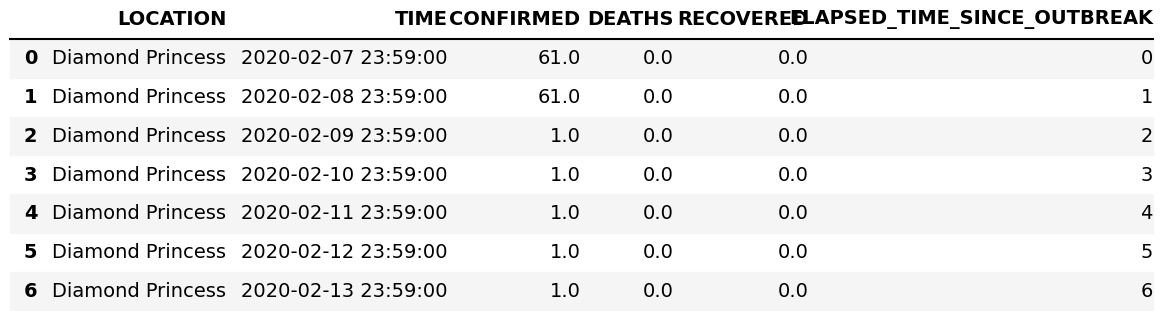
\includegraphics[width=1.0\linewidth]{fig-pandas/merge3.png}}
  \caption{
  Result of outer merging and summing. \label{fig:pandas:merge3}
  }
\end{figure}
%\clearpage % flush figures fig:pandas:merge3

\subsection{Working with folders and files}
When working with big data sets you might want to split data into smaller sets, and also write them to different folders (or files) to view each individually in excel. Working with files and folders in a way that will work on any kind of platform has always been a challenge, but it is greatly simplified by the \href{{https://docs.python.org/3/library/pathlib.html}}{Pathlib library}.

\paragraph{Basic use of Pathlib.}
\paragraph{List all sub directories and files:}









\begin{pro}{cbg_blue1}{bar_blue1}\begin{Verbatim}[numbers=none,fontsize=\fontsize{9pt}{9pt},baselinestretch=0.95,xleftmargin=2mm]
from pathlib import Path
p=Path('.') # the directory where your python file is located
for x in p.iterdir():
    if x.is_dir():
        print('Found dir: ', x)
    elif x.is_file():
        print('Found file: ', x)

\end{Verbatim}
\end{pro}
\noindent


\paragraph{List all files of a type:}




\begin{pro}{cbg_blue1}{bar_blue1}\begin{Verbatim}[numbers=none,fontsize=\fontsize{9pt}{9pt},baselinestretch=0.95,xleftmargin=2mm]
p=Path('.')
for p in p.rglob("*.png"):# rglob means recursively, searches sub directories
    print(p.name)

\end{Verbatim}
\end{pro}
\noindent

If you want to print the full path do \texttt{print(p.absolute())}.

\paragraph{Create a directory:}


\begin{pro}{cbg_blue1}{bar_blue1}\begin{Verbatim}[numbers=none,fontsize=\fontsize{9pt}{9pt},baselinestretch=0.95,xleftmargin=2mm]
Path('tmp_dir').mkdir()

\end{Verbatim}
\end{pro}
\noindent

If you run the code twice it will produce an error, because the directory exists, then we can simply do \Verb!Path('tmp_dir').mkdir(exist_ok=True)!.

\paragraph{Print current directory:}


\begin{pro}{cbg_blue1}{bar_blue1}\begin{Verbatim}[numbers=none,fontsize=\fontsize{9pt}{9pt},baselinestretch=0.95,xleftmargin=2mm]
Path.cwd()

\end{Verbatim}
\end{pro}
\noindent


\paragraph{Joining paths:}





\begin{pro}{cbg_blue1}{bar_blue1}\begin{Verbatim}[numbers=none,fontsize=\fontsize{9pt}{9pt},baselinestretch=0.95,xleftmargin=2mm]
p=Path('.')
new_path = p / 'tmp_dir' / 'my_file.txt'
print(new_path.absolute())
new_path.touch()

\end{Verbatim}
\end{pro}
\noindent


\paragraph{Basic use of \texttt{os}.}
We have already encountered the use of \texttt{os} when printing the working directory, i.e. \texttt{print(os.getcwd())}. If you want to create a directory named \texttt{tmp}, one can do

\paragraph{Creating a directory:}



\begin{pro}{cbg_blue1}{bar_blue1}\begin{Verbatim}[numbers=none,fontsize=\fontsize{9pt}{9pt},baselinestretch=0.95,xleftmargin=2mm]
import os
os.mkdir('tmp')

\end{Verbatim}
\end{pro}
\noindent

\paragraph{Moving into a directory:}
To move into that directory do



\begin{pro}{cbg_blue1}{bar_blue1}\begin{Verbatim}[numbers=none,fontsize=\fontsize{9pt}{9pt},baselinestretch=0.95,xleftmargin=2mm]
os.chdir('tmp')
os.chdir('..') # move back up

\end{Verbatim}
\end{pro}
\noindent


\paragraph{Splitting data into different folders and files.}
\paragraph{Using the Pathlib library:}












\begin{pro}{cbg_blue1}{bar_blue1}\begin{Verbatim}[numbers=none,fontsize=\fontsize{9pt}{9pt},baselinestretch=0.95,xleftmargin=2mm]
df=pd.read_excel('../data/corona_data.xlsx')
countries = df['LOCATION'].unique() #skip duplicates
data_folder=Path('../covid-data')
data_folder.mkdir()
for country in countries:
    new_path=data_folder / country
    new_path.mkdir()
    excel_file=country+'.xlsx'
    df2=df[df['LOCATION']==country]
    df2.to_excel(new_path/excel_file,index=False)

\end{Verbatim}
\end{pro}
\noindent

If you run the code twice, it will fail, but that can be resolved by e.g. \Verb!data_folder.mkdir(exist_ok=True)!.  

\paragraph{Using the \texttt{os} library:}













\begin{pro}{cbg_blue1}{bar_blue1}\begin{Verbatim}[numbers=none,fontsize=\fontsize{9pt}{9pt},baselinestretch=0.95,xleftmargin=2mm]
# first get all the countries:
df=pd.read_excel('../data/corona_data.xlsx')
countries = df['LOCATION'].unique() #skip duplicates
os.mkdir('../covid-data')
os.chdir('../covid-data')
for country in countries:
    os.mkdir(country)
    os.chdir(country)
    df2=df[df['LOCATION']==country]
    df2.to_excel(country+'.xlsx',index=False)
    os.chdir('..') # move up

\end{Verbatim}
\end{pro}
\noindent


More robust way of creating a directory







\begin{pro}{cbg_blue1}{bar_blue1}\begin{Verbatim}[numbers=none,fontsize=\fontsize{9pt}{9pt},baselinestretch=0.95,xleftmargin=2mm]
def my_mkdir(name):
    if os.path.isdir(name):
        print('Directory ', name,' already exists')
    else:
        os.mkdir(name)
        print('creating directory ',name)

\end{Verbatim}
\end{pro}
\noindent


If you want to collect all data, you can do as follows









\begin{pro}{cbg_blue1}{bar_blue1}\begin{Verbatim}[numbers=none,fontsize=\fontsize{9pt}{9pt},baselinestretch=0.95,xleftmargin=2mm]
df_new=pd.DataFrame()
data_folder=Path('../covid-data')
for dir in data_folder.iterdir():
    if dir.is_dir():      
        file=dir.name+'.xlsx'
        df=pd.read_excel(dir/file)
        print('Reading file ', file)
        df_new=pd.concat([df_new,df],ignore_index=True)

\end{Verbatim}
\end{pro}
\noindent


\subsection{Writing more robust code}
Most likely in the last sections you have encountered quite long error messages from Python. Errors could be
\begin{itemize}
\item syntax errors, grammatically incorrect code e.g.~calling functions that does not exists, using variables that are not defined or writing lines of codes with missing instructions, indentation errors 

\item exceptions e.g.~open a file that does not exists, accessing a Pandas header with the wrong name, performing wrong mathematical operations (1/0)

\item logical errors (bugs), code that runs but produces wrong results. These errors are of course some of the most difficult errors to fix and can only be discovered by comparing the output of the code to known answers. In many cases errors are introduced when extending the code, and unit tests can be extremely helpful.
\end{itemize}

\noindent
In the rest of this section we will discuss how to avoid or to handle exceptions. The goal is to write a code that catch all the exceptions before they happen, tries to do something with them, if not prints out a reasonable error message of what went wrong.

Let us look at the code that we have written so far, starting from the top of the notebook.

\paragraph{Accessing columns in Pandas:}
So far we have just accessed the columns directly, but it is very quick to write a wrong name, thus instead of doing


\begin{pro}{cbg_blue1}{bar_blue1}\begin{Verbatim}[numbers=none,fontsize=\fontsize{9pt}{9pt},baselinestretch=0.95,xleftmargin=2mm]
time=df['TIME']

\end{Verbatim}
\end{pro}
\noindent

we should try to check if the column exist before accessing it from the DataFrame. There are many ways of achieving this
















\begin{pro}{cbg_blue1}{bar_blue1}\begin{Verbatim}[numbers=none,fontsize=\fontsize{9pt}{9pt},baselinestretch=0.95,xleftmargin=2mm]
def get_column_from_dataframe(name,df):
    '''
    name: name of column
    df: Pandas DataFrame
    returns: column if found, and empty otherwise 
    '''
    if name in df.columns:
        return df[name]
    else:
        print('Column not found')
        print('Possible column names are : ', df.columns)
        return pd.Series(dtype=object)
# run the following code with df containing covid data
get_column_from_dataframe('TIME2',df)
get_column_from_dataframe('TIME',df)

\end{Verbatim}
\end{pro}
\noindent

Note the use of doc string in the beginning, the doc string will be printed in advanced editors once you write the name of the function. It also helps you to remember what the function does. It is a good practice to return something of the same type, because then the rest of the code can execute. If it is critical that you find the name of the column you can always test from the outside





\begin{pro}{cbg_blue1}{bar_blue1}\begin{Verbatim}[numbers=none,fontsize=\fontsize{9pt}{9pt},baselinestretch=0.95,xleftmargin=2mm]
s=get_column_from_dataframe('TIME2',df)
if s.empty:
    print('Exiting ...')
    exit() # note this shuts down the kernel

\end{Verbatim}
\end{pro}
\noindent

In the function \Verb!get_column_from_dataframe! many more things could go wrong, the user could pass a variable that is not a DataFrame, to catch all exceptions one can do















\begin{pro}{cbg_blue1}{bar_blue1}\begin{Verbatim}[numbers=none,fontsize=\fontsize{9pt}{9pt},baselinestretch=0.95,xleftmargin=2mm]
def get_column_from_dataframe_v2(name,df):
    '''
    name: name of column
    df: Pandas DataFrame
    returns: column if found, and empty otherwise 
    '''
    try:
        return df[name]
    except:
        print('Something went wrong ...')
        print('Maybe wrong column name?')
        return pd.Series(dtype=object)
# run the following code with df containing covid data
get_column_from_dataframe_v2('TIME2',df)

\end{Verbatim}
\end{pro}
\noindent

The \texttt{try} and \texttt{except} handling is very elegant in Python, and a very easy way of making the code more robust. Python first tries \texttt{df[name]} if that is not successful (e.g.~wrong column name, wrong DataFrame, maybe Pandas is not even imported) it jumps to the exception.

Another thing to consider is to use case insensitive search, we should be able to access a country or a header using e.g. \texttt{Afghanistan} or \texttt{afghanistan}. A possible solution could be to make sure that when you read in the 


















\begin{pro}{cbg_blue1}{bar_blue1}\begin{Verbatim}[numbers=none,fontsize=\fontsize{9pt}{9pt},baselinestretch=0.95,xleftmargin=2mm]
def get_column_from_dataframe_v3(name,df):
    '''
    name: name of column (case insensitive)
    df: Pandas DataFrame
    returns: column if found, and empty otherwise 
    '''
    COL=df.columns.str.upper()
    NAME=name.upper()
    try:
        idx=COL.get_loc(NAME)
        return df.iloc[:,idx]
    except:
        print('Column not found')
        print('Possible column names are : ', df.columns)
        return pd.Series(dtype=object)
        
get_column_from_dataframe_v3('time',df)

\end{Verbatim}
\end{pro}
\noindent

Now, we might want to make our code more robust when collecting data for e.g.~a specific country \texttt{df[df['LOCATION'] == 'Afghanistan']}. This operation assumes 1) that the column \texttt{LOCATION} exists and 2) that the country is spelled correctly. However, we have already written code to get a column and check that it exists, but it is written inside a function with a different purpose. Thus, it is better to split the code above in two parts










































\begin{pro}{cbg_blue1}{bar_blue1}\begin{Verbatim}[numbers=none,fontsize=\fontsize{9pt}{9pt},baselinestretch=0.95,xleftmargin=2mm]
def get_col_index(name,df):
    '''
    name: name of column (case insensitive)
    df: Pandas DataFrame
    returns: pos if exists, and -1 otherwise 
    '''
    COL=df.columns.str.upper()
    NAME=name.upper()
    try:
        return COL.get_loc(NAME)
    except:
        print('Column not found')
        print('Possible column names are : ', df.columns)
        return -1

def get_column_from_dataframe_v4(name,df):
    '''
    name: name of column (case insensitive)
    df: Pandas DataFrame
    returns: column if found, and empty otherwise 
    '''
    idx=get_col_index(name,df)
    if idx>-1:
        return df.iloc[:,idx]
    else:
        return pd.Series(dtype=object)
        
def get_rows_from_dataframe(name,df,col='LOCATION'):
    '''
    name: name of rows (case insensitive)
    df: Pandas DataFrame
    col: name of column to use as logical test
    returns: DataFrame, and empty otherwise 
    '''
    idx=get_col_index(col,df)
    if idx>-1:
        NAME=name.upper()
        return df[df.iloc[:,idx].str.upper() == NAME]
    else:
        return pd.DataFrame()
get_rows_from_dataframe('afGhaniStan',df)

\end{Verbatim}
\end{pro}
\noindent


\paragraph{To summarize:}

\begin{enumerate}
\item We want to catch errors before they occur, this is most efficiently done by wrapping simple operations in functions

\item Functions should be small, i.e.~only to as little as possible, that would increase their reusability

\item Almost all exceptions can be caught by using \texttt{try} and \texttt{except} functionality in Python

\item Write doc strings in functions to increase user friendliness

\item Write meaningful error messages, if possible also print out some additional information to help the user 
\end{enumerate}

\noindent
\bibliographystyle{plain}
\bibliography{../papers}


% ------------------- end of main content ---------------

% #ifdef PREAMBLE
\end{document}
% #endif

